\chapter{Przegląd istniejących rozwiązań}
	Procesor Zilog Z80 jest często emulowany, ze względu na jego dużą popularność. Emulatory tworzone są zarówno przez duże firmy, jak i hobbystów. Na platformie \emph{Github}  która jest przeznaczona dla projektów programistycznych, można znaleźć około dwustu repozytoriów z projektami emulującymi Z80, lub urządzenia używające tego procesora. %\cite{githubZ80Emulators}

	W~tym rozdziale zaprezentowane są najciekawsze emulatory, które posiadają graficzny interfejs użytkownika i pozwalają na wgląd w wewnętrzne stany procesora (czyli najbardziej przypominające zakresem swoich funkcji aplikację będącą przedmiotem tej pracy). Przedstawione są zarówno komercyjne rozwiązania, jak i te pisane przez amatorów.
	
	\section{Z80 SIMULATOR IDE}
	Jest to dostępny pod adresem http://www.oshonsoft.com/z80.html płatny emulator posiadający najbardziej rozbudowany interfejs z wszystkich opisanych programów. 
	Pozwala on na prezentowanie wewnętrznych stanów procesora, manipulację przerwaniami i portami wejścia/wyjścia. Zawiera edytor pamięci działający również podczas emulacji. 
	Posiada on również funkcje i~elementy typowe dla debuggerów, jak możliwość wstrzymania działania programu w określonym miejscu, tryb pracy krokowej, interaktywny edytor i~kompilator kodu asemblera\cite{oshonsoftEmulator}. Widok interfejsu użytkownika tego programu jest zaprezentowany na rysunku \ref{img:oshonsoftEmulator}.
	
	\begin{figure}[h]
		\centering
		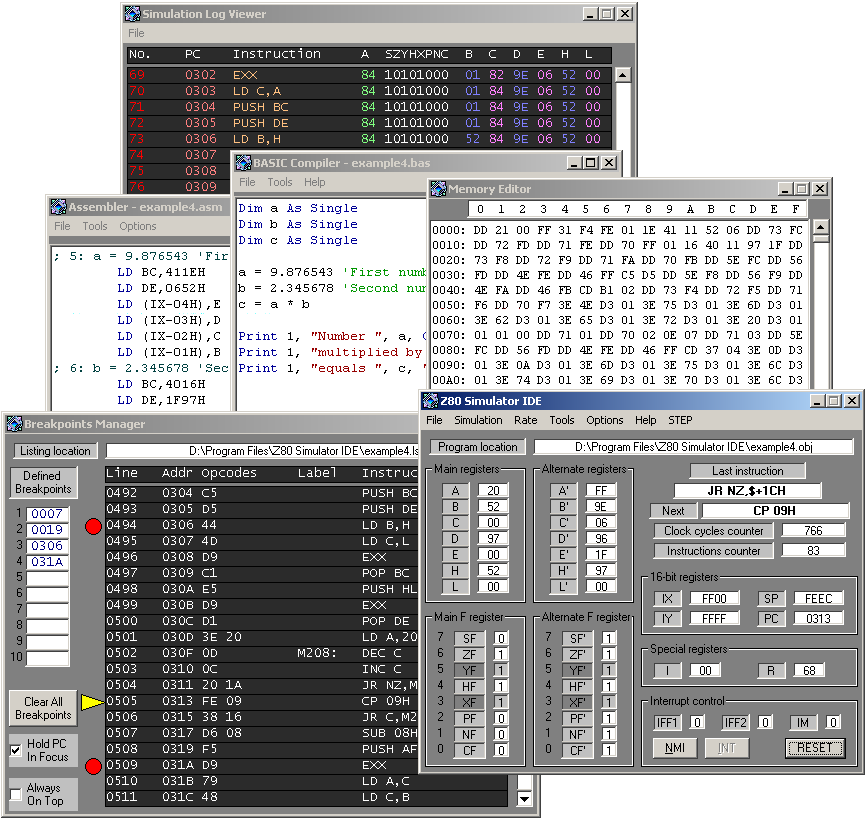
\includegraphics[width=0.7\textwidth]{oshonsoftEmulator}
		\caption{Z80 SIMULATOR IDE}
		\label{img:oshonsoftEmulator}
	\end{figure}
	
	Jedną z wad emulatora Z80 SIMULATOR IDE jest interfejs, który nie jest intuicyjny. Przykładowo, autorzy programu nie umieścili w~nim informacji, o tym w jakim formacie powinny być wprowadzane wartości liczbowe. Brak w programie systemu pomocy i opisów, co może znacznie utrudniać pracę początkującym użytkownikom. Dodatkowo jest to narzędzie płatne, przeznaczone dla specjalistów i~uruchamiane tylko w~systemie MS Windows.
	
	
	\section{ZEMU - Z80 Emulator Joe Moore}
	ZEMU to emulator zaprojektowany głównie po to, aby umożliwiać uruchamianie systemu operacyjnego CPM, który był oferowany przez firmę \emph{Digital Research Inc.} w~latach 1970{\dywiz}1980\cite{cpm}. Program skierowany jest do hobbystów. Oprócz standardowych możliwości takich jak podgląd, edycja zawartości pamięci, rejestrów i flag, może on również emulować stację dyskietek, port COM, szeregowy, monitor CRT i~drukarkę.    
	
	Rysunek \ref{img:zemu} przedstawia interfejs aplikacji. Tak, jak w przypadku Z80 SIMULATOR IDE nie jest on intuicyjny, brak mu systemu pomocy, jego elementy nie są opisane w wystarczającym stopniu. Osoby nie mające doświadczenia z urządzeniami wejścia/wyjścia w Zilogu Z80 będą miały problem z obsługą nawet podstawowych funkcji.
	
	Inną wadą aplikacji jest brak możliwości jej uruchomienia w~innym systemie operacyjnym niż \emph{Windows}. 
	
	\begin{figure}[h]		
		\centering
		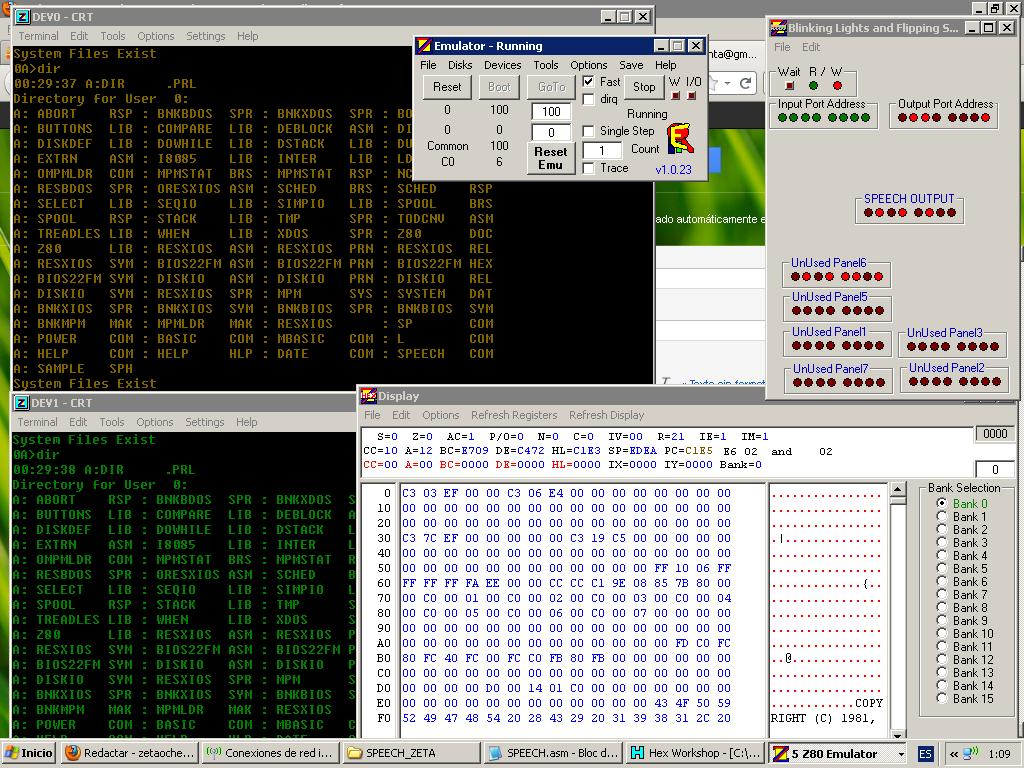
\includegraphics[width=0.8\textwidth]{zemu}
		\caption{ZEMU}
		\label{img:zemu}
	\end{figure}
	
	 \section{ZIM - The Z80 Machine Simulator}
	ZIM został napisany z~użyciem technologii \emph{Java Web-Start}. Pozwala ona na uruchomienie aplikacji bezpośrednio na stronie internetowej, ale również pozwala na dostęp do lokalnych zasobów komputera, np. plików. 
	Aplikacja według autora przeznaczona jest głównie dla studentów uczących się języka asemblera dla procesora Z80\cite{zimManual}.
	
	Program pozwala na podgląd wszystkich wewnętrznych parametrów CPU, emuluje proste urządzenia wejścia/wyjścia, umożliwia edycję zawartości pamięci, debugowanie programu dla procesora Z80 i~symulację przerwań. Zaletą emulatora jest możliwość jego uruchamiania na wielu platformach sprzętowych, dzięki zastosowaniu języka Java.
	
	W~aplikacji brakuje natomiast edytora asemblera i~systemu pomocy. Interfejs użytkownika ma wiele defektów i nie jest intuicyjny. Na rysunku \ref{img:zim} przedstawiono zrzut ekranu działającej aplikacji.
	
	\begin{figure}[h]		
		\centering
		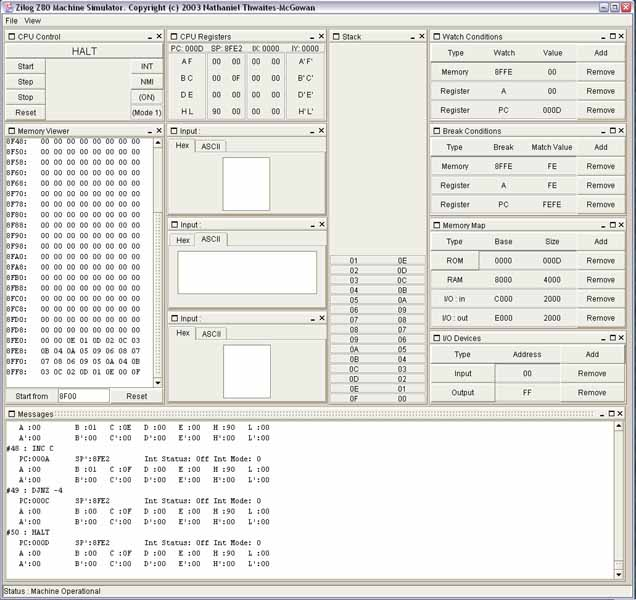
\includegraphics[width=0.8\textwidth]{zim}
		\caption{ZIM - The Z80 Machine Simulator}
		\label{img:zim}
	\end{figure}
	
	%Żadne istniejące rozwiązanie nie pozwala na podejrzenie wewnętrznych magistrali procesora
	
	\section{Podsumowanie istniejących rozwiązań}
	Problemem prawie wszystkich emulatorów i symulatorów jest ich interfejs użytkownika. Ta uwaga dotyczy nie tylko emulatorów konkretnie omawianego procesora, ale ogółu tego typu aplikacji. Są one przeznaczone dla osób znających architekturę komputerową, oraz budowę i działanie konkretnego emulowanego urządzenia. Z~tego powodu programiści nie przywiązują odpowiedniej wagi do intuicyjności i systemów pomocy dla interfejsów użytkownika. Osoby nieposiadające wymaganej wiedzy albo znające jedynie podstawy zagadnienia nie są w stanie sprawnie obsługiwać programu. 
	
	Emulatory nie są przeznaczone do uruchamiania na wielu platformach sprzętowych. Dotyczy to szczególnie aplikacji emulujących przez rekompilację. Do jej wykonania wymagana jest znajomość architektur wyjściowej i docelowej maszyny. Rozwiązaniem tego problemu mogą być interpretery napisane w języku Java, takie jak ,,ZIM - The Z80 Machine Simulator". Rozwiązanie to wykorzystuje dużo zasobów procesora. Kod przeznaczony dla emulowanej maszyny jest najpierw interpretowany przez interpreter napisany w języku Java, a następnie ponownie emulowany już za pomocą dynamicznej rekompilacji w maszynie wirtualnej. Typowe rozwiązania napisane w języku kompilowanym dla konkretnego procesora działają szybciej, kosztem możliwości uruchamiania na wielu platformach sprzętowych. Wydajność maszyny wirtualnej języka Java nie jest przeszkodą do stworzenia w~tym języku emulatora procesora Zilog Z80. Współczesne komputery są na tyle efektywne, że taki emulator może pracować z~wydajnością zbliżoną do wydajności oryginalnej maszyny.
	
	Kolejną kwestią o której warto wspomnieć jest czytelność kodu emulatorów. Kod istniejących rozwiązań nie należy do łatwych do zrozumienia. Najczęściej cały program w~postaci źródłowej emulatora zawiera się w jednym pliku o~wielkości kilkuset wierszy. Osoba chcąca przestudiować proces emulacji ma zatem utrudnione zadanie.
	
	Podsumowując, aktualnie brakuje wieloplatformowego emulatora lub symulatora Ziloga Z80, z czytelnym, poprawnie działającym interfejsem użytkownika, czytelnym, dobrze opisanym kodem źródłowym i~użytecznym systemem pomocy.
	